\documentclass[a4paper,twoside,12pt]{article}
\usepackage[T1]{fontenc}
\usepackage[utf8]{inputenc}
\usepackage[english]{babel}
%\usepackage[english=nohyphenation]{hyphsubst} % Tällä englannin tavutus pois.
%\usepackage[sc]{mathpazo} % Vaihtoehtoinen Palatino-fontti käyttöön.
\usepackage{enumerate}
\usepackage[shortlabels]{enumitem}
\usepackage{fullpage}
\usepackage{setspace}
\usepackage{graphicx}
\usepackage{import}
\usepackage{amsmath}
\usepackage{mathabx}
\usepackage{icomma}
\usepackage{booktabs}
\usepackage{ftcap}
\usepackage{lipsum}
\usepackage{url}
\usepackage{siunitx}
\usepackage{epstopdf}
\usepackage{hyperref}

\begin{document}
\onehalfspacing%  % Riviväli 1.5.
\thispagestyle{empty}
\begin{flushleft}
 \underline{Sakari} Matias Kapanen\hfill
 \texttt{sakari.m.kapanen@student.jyu.fi}
\end{flushleft}
\vfill
\begin{center}
\textsc{\LARGE FYSS430 A computer tomographic study of the infill ratio of a 3D printed object}
\end{center}
\vfill
Measurement date: January 25, 2017\\
Supervisor: Arttu Miettinen\\
\vfill
\begin{abstract}
 \noindent
    TODO
\end{abstract}
\clearpage%

\setlength{\parindent}{0pt}  % Kappaleen alkuun ei sisennystä.
\setlength{\parskip}{12pt}  % Sen sijaan kappaleiden väliin rako.

\setcounter{page}{1}

\section{Introduction}
Three-dimensional printing is an additive manufacturing method where plastic is extruded layer by layer to produce a three-dimensional object. A solid 3D CAD model is prepared for printing by a ``slicer'' software which generates the tool paths for the nozzle.

It does not often make sense to fill the whole solid model with plastic. Therefore a sparse ``infill'' pattern is generated instead as shown in image~\ref{fig:honeycomb}.

The volumetric ratio of the infill material inside the cube was chosen as the research subject of this computer tomography project work. Tomographic imaging makes it possible to acquire a volume image of the 3D printed cube which can be then analyzed by traditional image analysis methods.

\begin{figure}
    \centering
    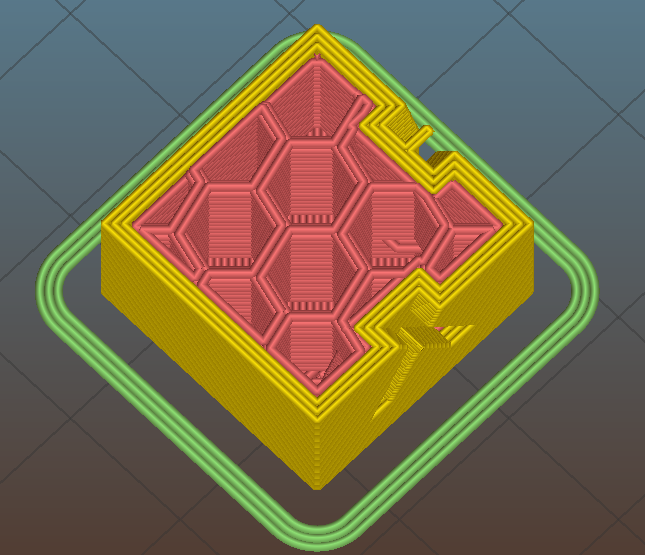
\includegraphics[width=0.8\textwidth]{images/cube_slic3r.png}
    \caption{A section of a three-dimensional cube model~\cite{testcube} sliced by Slic3r~\cite{slic3r}. A honeycomb infill pattern of 20 \% ratio has been generated inside.}
    \label{fig:honeycomb}
\end{figure}

\section{Theoretical background}
In this section, the theoretical foundations of computer tomographic imaging and image reconstruction are lightly covered. There is also a brief introduction to the image processing methods used.

In typical X-ray tomography scenarios, an X-ray beam is cast on the object to be imaged. On the other side there is a detector array. The object is mounted on a rotation stage. This allows taking X-ray projections of the object from different directions. From the two-dimensional projections, a volume image can be reconstructed.

\subsection{Beer-Lambert law}
The X-ray beams enterig the target object are attenuated in the material. The attenuation can be attributed to various scattering phenomena taking place in the medium, most importantly photoelectric effect and Compton scattering~\cite{lectures}. The probaility of these scatterings correlates to the density of the target material.

Consider a beam propagating in one dimension. In a simple linear model, the rate of the scatterings is proportional to the attenuation coefficient $\mu(x)$ and the beam intensity $I(x)$. On the other hand, the scatterings decrease the intensity. Therefore the change of intensity with respect to traveled distance can be written as
\begin{equation}
    \label{eq:bl_ode}
    \frac{\mathrm{d}I(x)}{\mathrm{d}x} = -\mu (x) I (x).
\end{equation}
This differential equation has a familiar solution of the form
\begin{equation}
    \label{eq:bl}
    I(x) = I_0 e ^ { -\int\limits_0^x \mu(x)\,\mathrm{d}x },
\end{equation}
where $I_0$ is the initial beam intensity. In the special case of a uniform medium, this becomes
\begin{equation}
    \label{eq:bl_linear}
    I(x) = I_0 e ^ { -\mu x }.
\end{equation}
Therefore it is seen that the beam exponentially decays in the medium. The thickness and the density of the medium therefore both contribute to the attenuation.

\subsection{Filtered backprojection}
Given a sufficient number of $Z$-projections, one can costruct an image of the original volume. A simple method is to algebraically solve for the original voxel values using the projection data. However, this is inconvenient for any practical image sizes because the resulting equation group is large.

A more widely used, practical method is filtered backprojection. It is an integral transform based approach which is described in detail in~\cite{radon}. The basic idea is as follows:
\begin{enumerate}
    \item Each $Z$-slice is processed individually. The \emph{rows} of the projection images are considered as the projections of the respective slices, situated in the $XY$ plane.

    \item The series of projections of a single slice at different rotation angles are considered as the Radon transform of the slice.

    \item The Radon transform data is filtered in the Fourier plane by a filter $h(\omega) = |\omega|$. This step has a high pass filtering effect and arises from the mathematics of the Radon transform.

    \item The filtered data is transformed with the inverse Radon transform. The result of the inverse transform is an image of the corresponding $Z$-slice.

    \item The procedure 2-4 is repeated for all slices, resulting in a volume image.
\end{enumerate}

Often, after the reconstruction process, the voxel values of the result are inverted such that larger values (brighter regions) correspond to volumes of greater density.

\subsection{Binary images and thresholding}
The volume image recovered by the reconstruction process is a greyscale image. To analyze different sections of the image, some kind of \emph{segmentation} has to be performed. One of the simplest cases of segmentation is the extraction of a light foreground from a dark background. In a simple case, the result of such an operation is a binary image where the foreground pixels are marked white and background pixels are marked black.

A binary mask like that can be achieved by thresholding: given a threshold value $t$, the thresholded image is given by
\begin{equation}
    \label{eq:threshold}
    g_t(\mathbf{x}) = \begin{cases}
        0 & \text{where } f(\mathbf{x}) \geq t \\
        1 & \text{where } f(\mathbf{x}) < t,
    \end{cases}
\end{equation}
where $f(\mathbf{x})$ is the original image. The thresholded image $g_t(\mathbf{x})$ has only values 0 and 1 and is thus called a \emph{binary} image.

The problem now boils down to finding the optimal threshold value which actually separates the foreground from the background. There are several automatic methods for obtaining such a threshold. One of them is the Otsu method~\cite{otsu}. I this method, the threshold is found as a solution to the optimization problem
\[
    \sigma_\text{B}^2(t_\text{Otsu}) = \max\limits_t \sigma_\text{B}^2(t),
\]
where $\sigma_\text{B}^2(t)$ is the between-class variance of the background and foreground pixel (or voxel) values of the respective pixel classes separated by the threshold $t$. This method works well if there are clear foreground and background peaks in the image histogram.

\subsection{Edge detection}
Another commonly useful image processing operation is edge detection. The notion of an edge usually corresponds to a discontiuity or a rapid change in the image. Therefore partial derivatives of the image are a natural way of finding derivatives.

However, derivatives are also sensitive to noise in the image. Some low pass filtering of the image is usually performed to reduce noise. A useful property of convolution allows combining the derivative and the convolution operations:
\begin{equation}
    \frac{\partial}{\partial x} (f(x, y) \ast \mathbf{G}_\sigma) =
    f(x, y) \ast \frac{\partial}{\partial x} \mathbf{G}_\sigma,
\end{equation}
where $\mathbf{G}_\sigma$ is the Gaussian kernel with the width parameter $\sigma$ and $\ast$ is convolution. Thus, combined edge detection and low pass filtering can be done by convolving the image with kernel approximating the partial derivatives of the Gaussian function.

One can derive edge detection kernels of arbitrary sizes and accuracies. The Sobel kernels are a widely used approximation:
\begin{equation}
    \mathbf{G}_x = \begin{bmatrix}
        -1 & 0 & 1 \\
        -2 & 0 & 2 \\
        -1 & 0 & 1
    \end{bmatrix},
    \mathbf{G}_y = \begin{bmatrix}
        -1 & -2 & -1 \\
        0 & 0 & 0 \\
        1 & 2 & 1
    \end{bmatrix},
\end{equation}
which, while not greatly accurate, are an acceptable opinion if the desired result is achieved.

Given the values of the $x$ and $y$ partial derivatives, the magnitude of the gradient can be calculated as
\[
    \mathbf{G} = \sqrt{\mathbf{G}_x^2 + \mathbf{G}_y^2}.
\]
High values of the gradient magnitude signify the image edges.

\subsection{Morphological operations}
Morphological operations are a set of mathematical operations on binary images. The basic operations are \emph{erosion}, \emph{dilation}, \emph{opening} and \emph{closing}. All these operations involve the usage of a \emph{structuring element} which is a $n$-by-$m$ binary mask which determines the neighbourhood that is sampled for each pixel during the operation.

Erosion and dilation are complementary: erosion shrinks white regions in the source image, dilation expands them (or shrinks black regions).

Opening is the chained operation of an erosion followed by a dilation. This removes white regions smaller than a certain size. Closing is the complement, which removes black regions smaller than a certain size.

These operations are widely implemented in popular image processing libraries and useful in manipulating binary images. For a more thorough explanation of them, see e.g. the OpenCV documentation~\cite{cv1, cv2}.

\section{Experimental methods}
\subsection{SkyScan 1172 CT scanner}

\subsection{Image analysis software}

\section{Results}

\section{Conclusions}

\clearpage

\begin{thebibliography}{9}
    \bibitem{testcube} XYZ 20mm Calibration Cube. User \emph{iDig3Dprinting}. \url{http://www.thingiverse.com/thing:1278865}. Referenced March 7, 2017.

    \bibitem{slic3r} Slic3r, G-code generator for 3D printers. \url{http://slic3r.org/}. Referenced March 7, 2017.

    \bibitem{lectures} FYSS430 X-ray tomography and image analysis, lecture notes. \emph{Arttu Miettinen}. University of Jyväskylä, 2017.

    \bibitem{radon} Applied Fourier Analysis and Elements of Modern Signal Processing, lecture notes. \emph{Emmanuel Candes}. Stanford University, 2016. \url{http://statweb.stanford.edu/~candes/math262/Lectures/Lecture09.pdf}. Referenced March 7, 2017.

    \bibitem{otsu} A Threshold Selection Method from Gray-Level Histograms. \emph{Nobuyuki Otsu}. IEEE Transactions on systems, man and cybernetics, vol. SMC-9, no. 1. January 1979.

    \bibitem{cv1} Eroding and Dilation. OpenCV 2.4.13 documentation. \url{http://docs.opencv.org/2.4/doc/tutorials/imgproc/erosion_dilatation/erosion_dilatation.html?highlight=morphology}. Referenced March 7, 2017.

    \bibitem{cv2} More Morphology Transformations. OpenCV 2.4.13 documentation. \url{http://docs.opencv.org/2.4/doc/tutorials/imgproc/opening_closing_hats/opening_closing_hats.html?highlight=morphology}. Referenced March 7, 2017.
\end{thebibliography}
\end{document}

